\documentclass[12pt,a4paper]{abnt}
\usepackage[utf8]{inputenc}
\usepackage[T1]{fontenc}
\usepackage[english,brazilian]{babel}
\usepackage{hyperref}
\usepackage{url}
\usepackage{indentfirst}
\hypersetup{%
    pdfborder = {0 0 0}
}
\usepackage{graphicx}
\graphicspath{{./images/}}
\usepackage{placeins}
\newcommand{\Protocolo}[3]{
	\noindent Comando: \textbf{#1} \\
	Função: #2 \\
	Respostas: \\ #3
}
\newcommand{\ProtocoloResposta}[2]{
 \textbf{#1} - #2\\
}



\begin{document}

\chapter{Introdução}
	\section{Visão Geral}
		O sistema distribuído proposto tem o objetivo de paralelizar o uso de um \emph{WPA cracker}, no caso \emph{aircrack}, para que possa-se alcançar um desempenho melhor na realização de quebra de uma chave WPA-PSK. Com uma arquitetura cliente-servidor, 
		temos um computador servidor que tem o papel de coordenar a distribuição de tarefas entre vários clientes. Os computadores clientes recebem as tarefas do servidor, executam e retornam informações sobre o andamento quando solicitado pelo servidor.
		
		\subsection{Atividades do Servidor}
		\begin{itemize}
			\item Fazer leitura do arquivo contendo um \emph{handshake} e transferir para os clientes 
			\item Realizar a divisão do dicionário de palavras para os clientes disponíveis
			\item Inicializar o processo de \emph{cracking}
			\item Monitorar o andamento de todos os clientes
		\end{itemize}
		
		\subsection{Atividades do Cliente}
		\begin{itemize}
			\item Receber o pacote capturado contendo um \emph{handshake}
			\item Gerar seu próprio dicionário de palavras baseado nas informações fornecidas pelo servidor
			\item Executar o \emph{cracker} e obter informações sobre o processo
		\end{itemize}

	\clearpage
	\section{Protocolo}

		\Protocolo{STATUS}
		{Solicita a situação atual do processo de um cliente}
		{
			\ProtocoloResposta{NOT\_STARTED}{O processo não foi iniciado}
			\ProtocoloResposta{PROCESSING}{O processo está em andamento}
			\ProtocoloResposta{FAILED}{Informa que houve uma falha no processo}
			\ProtocoloResposta{KEY\_FOUND}{Informa que o processo foi finalizado e a palavra chave foi encontrada com sucesso}
			\ProtocoloResposta{KEY\_NOT\_FOUND}{Informa que o processo foi finalizado e a palavra chave não foi encontrada}
		}

		\Protocolo{CURRENT\_PASSPHRASE}
		{Solicita a um cliente qual \emph{passphrase} está atualmente sendo testada}
		{
			\ProtocoloResposta{CURRENT\_PASSPHRASE <passphrase>}{Informa a \emph{passphrase} atual}
		}

		\Protocolo{CURRENT\_TIME}
		{Solicita a um cliente o tempo decorrente do processo}
		{
			\ProtocoloResposta{CURRENT\_TIME <tempo>}{Informa o tempo decorrente do processo de um cliente}
		}
		
		\Protocolo{CURRENT\_KEYS\_PER\_SECOND}
		{Solicita a um cliente o número de chaves por segundo que está sendo tentado}
		{
			\ProtocoloResposta{CURRENT\_KEYS\_PER\_SECOND <keys>}{Informa o número de chaves por segundo}
		}
		
		\Protocolo{KEY\_FOUND}
		{Solicita a um cliente a chave encontrada}
		{
			\ProtocoloResposta{KEY\_FOUND <chave>}{Informa a chave encontrada}
		}
		
		\Protocolo{STOP\_CRACK}
		{Solicita a imediata interrupção do processo em um cliente}
		{
			\ProtocoloResposta{STOP\_OK}{Informa que o processo foi interrompido com sucesso}
			\ProtocoloResposta{STOP\_FAILED}{Informa que não foi possível interromper o processo}
		}
		
		\Protocolo{START\_CRACK <charset> <min> <max> <part> <cap>}
		{Solicita a inicialização do processo em um cliente}
		{
			\ProtocoloResposta{START\_OK}{Informa que o processo foi iniciado}
		}
		\clearpage
		\section{Diagrama de Caso de Uso}

		\begin{figure}[htp]
			\begin{center}
			  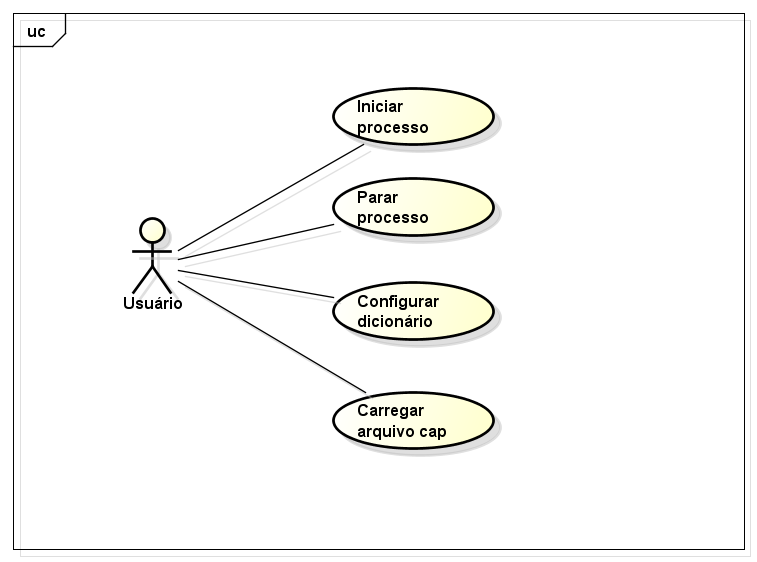
\includegraphics[width=350px]{casoDeUso}
			  \caption[Diagrama de Caso de Uso]{Diagrama de Caso de Uso}
			  \label{fig:casoDeUso}
			\end{center}
		\end{figure}
		\FloatBarrier

		\clearpage
		\section{Diagrama de Classes}

			\begin{figure}[htp]
				\begin{center}
				  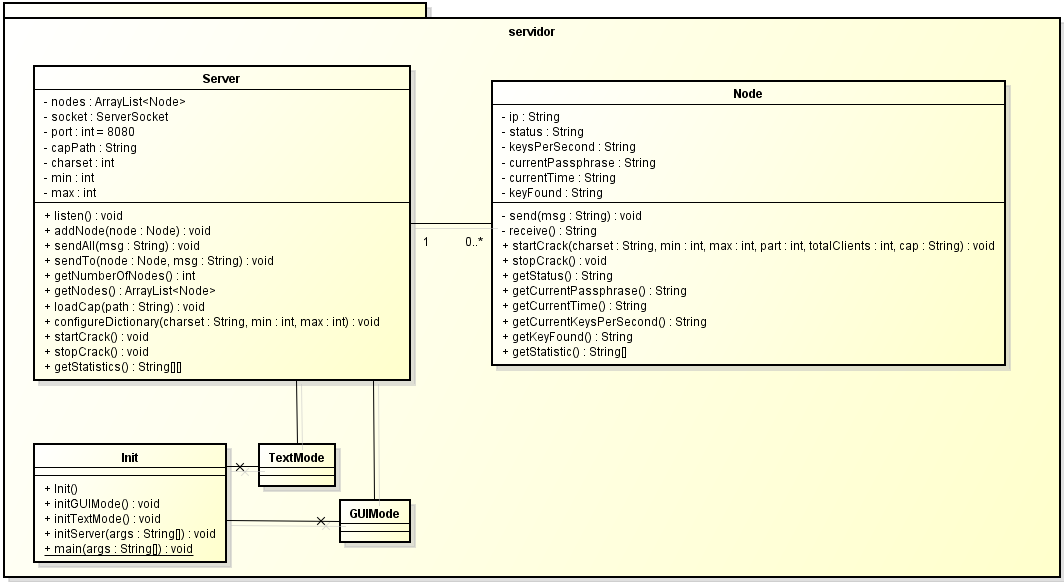
\includegraphics[width=350px]{diagramaClassesServidor}
				  \caption[Diagrama de Classes Servidor]{Diagrama de Classes Servidor}
				  \label{fig:diagramaClassesServidor}
				\end{center}
			\end{figure}
			\FloatBarrier

			\begin{figure}[htp]
				\begin{center}
				  \includegraphics[width=350px]{DiagramaClassesCliente}
				  \caption[Diagrama de Classes Cliente]{Diagrama de Classes Cliente}
				  \label{fig:diagramaClassesCliente}
				\end{center}
			\end{figure}
			\FloatBarrier

		\section{Diagrama de Sequencia}
		


\end{document}